\documentclass{article}

\usepackage{geometry}
\geometry{margin=2cm}
\usepackage{graphicx}
\usepackage{hyperref}
\usepackage{amsfonts}

\hypersetup{colorlinks=true, linkcolor=blue, urlcolor=blue}
\urlstyle{same}
\begin{document}
	
	\author{Aayush Arya}
	\date{(Submitted: \today)}
	\title{}
	
	\maketitle
	
	\hrule
	\begin{center}
		PHY366 Lab Report\\
		Practical: 3 \quad Registration No.: 11912610 \quad Section: G2903
	\end{center}
	\hrule
	
	\section*{Aim}
	To simulate and test differentiator and integrator circuits built using operational amplifiers.
	
	\section*{Methods}
	
	We simulate our operational amplifier circuit on the \textsc{MultiSim} platform. First, we constructed an integrator circuit that was input a $1V$ sinusoidal waveform with frequency 1 kHz\footnote{Integrator Circuit available publicly at \url{https://www.multisim.com/content/GnPE4shTsE3Pyz5586DRWd/integrator-circuit/open/}}
	(see Figure \ref{fig:circuit}).
	
	\begin{figure}[h!]
		\centering
		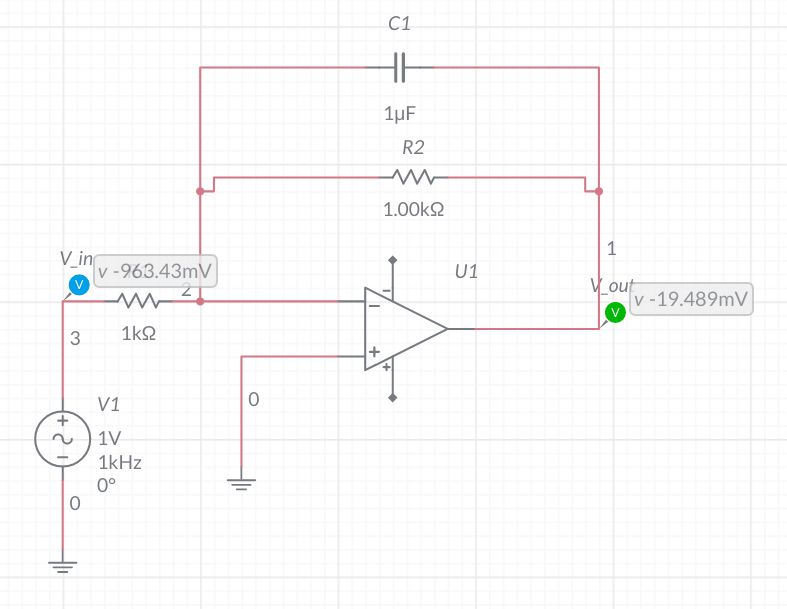
\includegraphics[width=0.6\textwidth]{integrator_circuit}
		\caption{Construction of an integrator circuit on MultiSim using an Op-Amp.}
		\label{fig:circuit}
	\end{figure}
	
	For an input of the form $ V_{in} = \sin \omega t$, one would expect to get a $V_{out} = \int\sin \omega t dt = -\cos \omega t$. We verify that this result is obtained in \nameref{sect:results}.\\\
	
	
 We also simulated a differentiator circuit using the same platform\footnote{Differentiator circuit available at \url{https://www.multisim.com/content/3q7Fr8CRbYhzxEkQLsXVHi/differentiator-circuit/open/}} (see Figure \ref{fig:diff_circuit}). In this circuit, the input that we provided was a $1V$ triangular wave. Such an input waveform has a shape corresponding to
 
 $$ f(t) = \left\{ 
 				\begin{array}{llr}
 					t &  &  0 < t < T/2\\
 					T- t &  & T/2 < t < T\\
 				\end{array}
 		\right\}$$
 
 And correspondingly, its derivative $$ f'(t) = 
		 \left\{
		 			\begin{array}{llr}
		 				1 &  & 0 < t < T/2\\
		 				-1 & & T/2 < t < T\\
		 			\end{array}
		 \right\}$$
		 
		 is expected to be a square wave. We test the validity of this prediction using the circuit illustrated in Figure \ref{fig:diff_circuit}.
 
 \begin{figure}[h!]
 	\centering
 	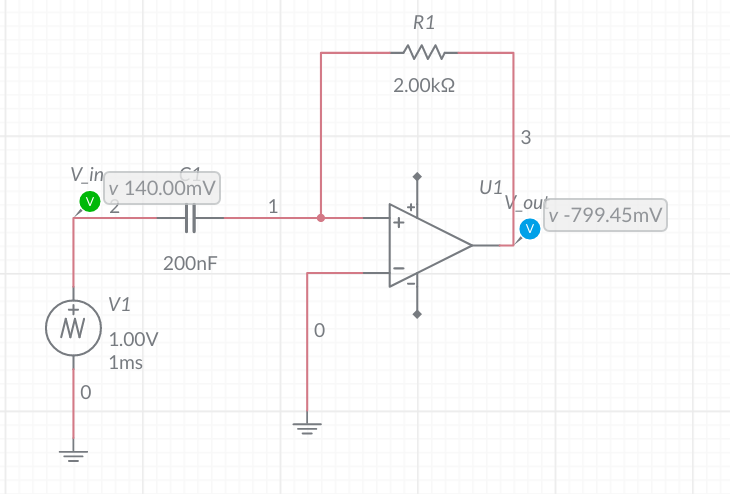
\includegraphics[width=0.5\textwidth]{diff_circuit}
 	\caption{Schematic of a differentiator circuit built using a 5-terminal Op-Amp}
 	\label{fig:diff_circuit}
 \end{figure}
	
	\section*{Results and Discussion}
	\label{sect:results}
	
	For the integrator circuit, the a portion of the response to the sinusoid has been shown in figure \ref{fig:integ_result}. Relevant data and plotting scripts have been enclosed along with this manuscript. \\
	
	\textbf{Note}: Due to a likely error in the export feature of the platform used, the scales of the x- and y- data have become interchanged, which affects Figure \ref{fig:integ_result}. A similar problem showed up for the differentiator circuit but could be resolved. We have not modified the data. We also note however, that the version of figure \ref{fig:diff_circuit} exported from the simulator itself {\bf did not} have these issues (see {\tt diff\_result\_multisim.png} provided with the manuscript).
	
	\begin{figure}[h!]
		\centering
		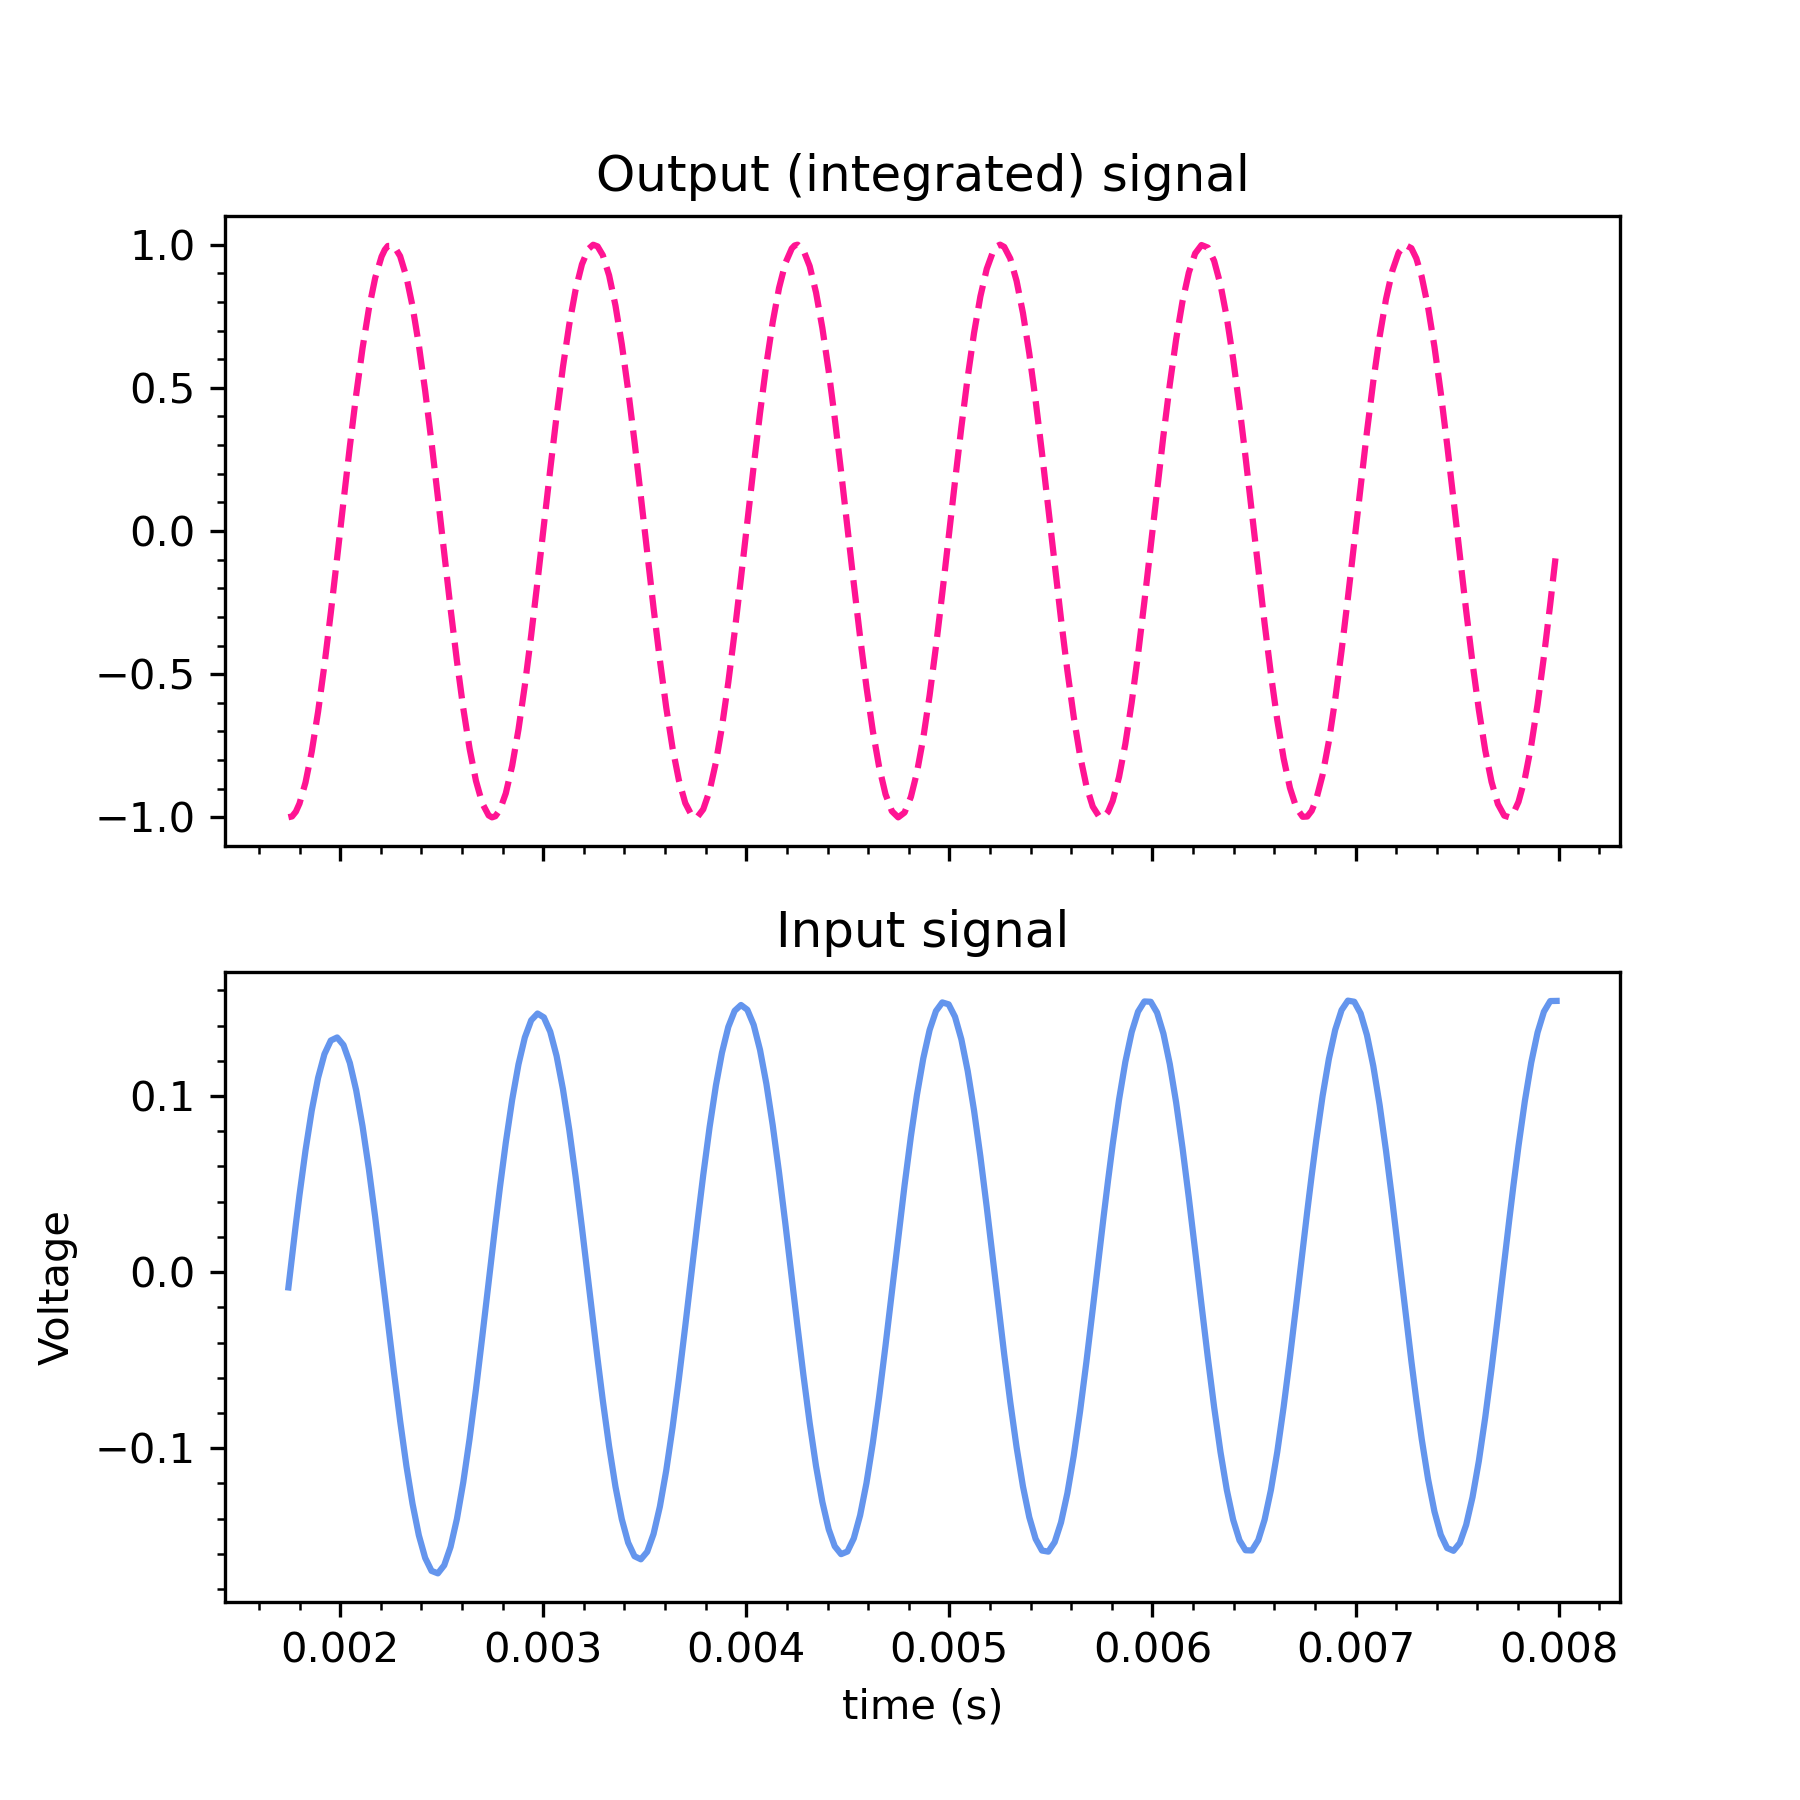
\includegraphics[width=0.4\textwidth]{integrator_result}
		\caption{A portion of the output response of the circuit along with the input signal itself. Note that the scale of the y-axes of the input and output voltages have been interchanged, likely due to an error in the \textsc{MultiSim} data export feature.}
		\label{fig:integ_result}
	\end{figure}
	
	Therefore, the result $\int \sin \omega t = - \cos \omega t$ is produced by the integrator as expected.\\
	
	Also, for the differentiator circuit, the output voltage for a triangular input waveform turns out to be a square wave (as expected, see Figure \ref{fig:diff_result}).
	
	\begin{figure}[h!]
		\centering
		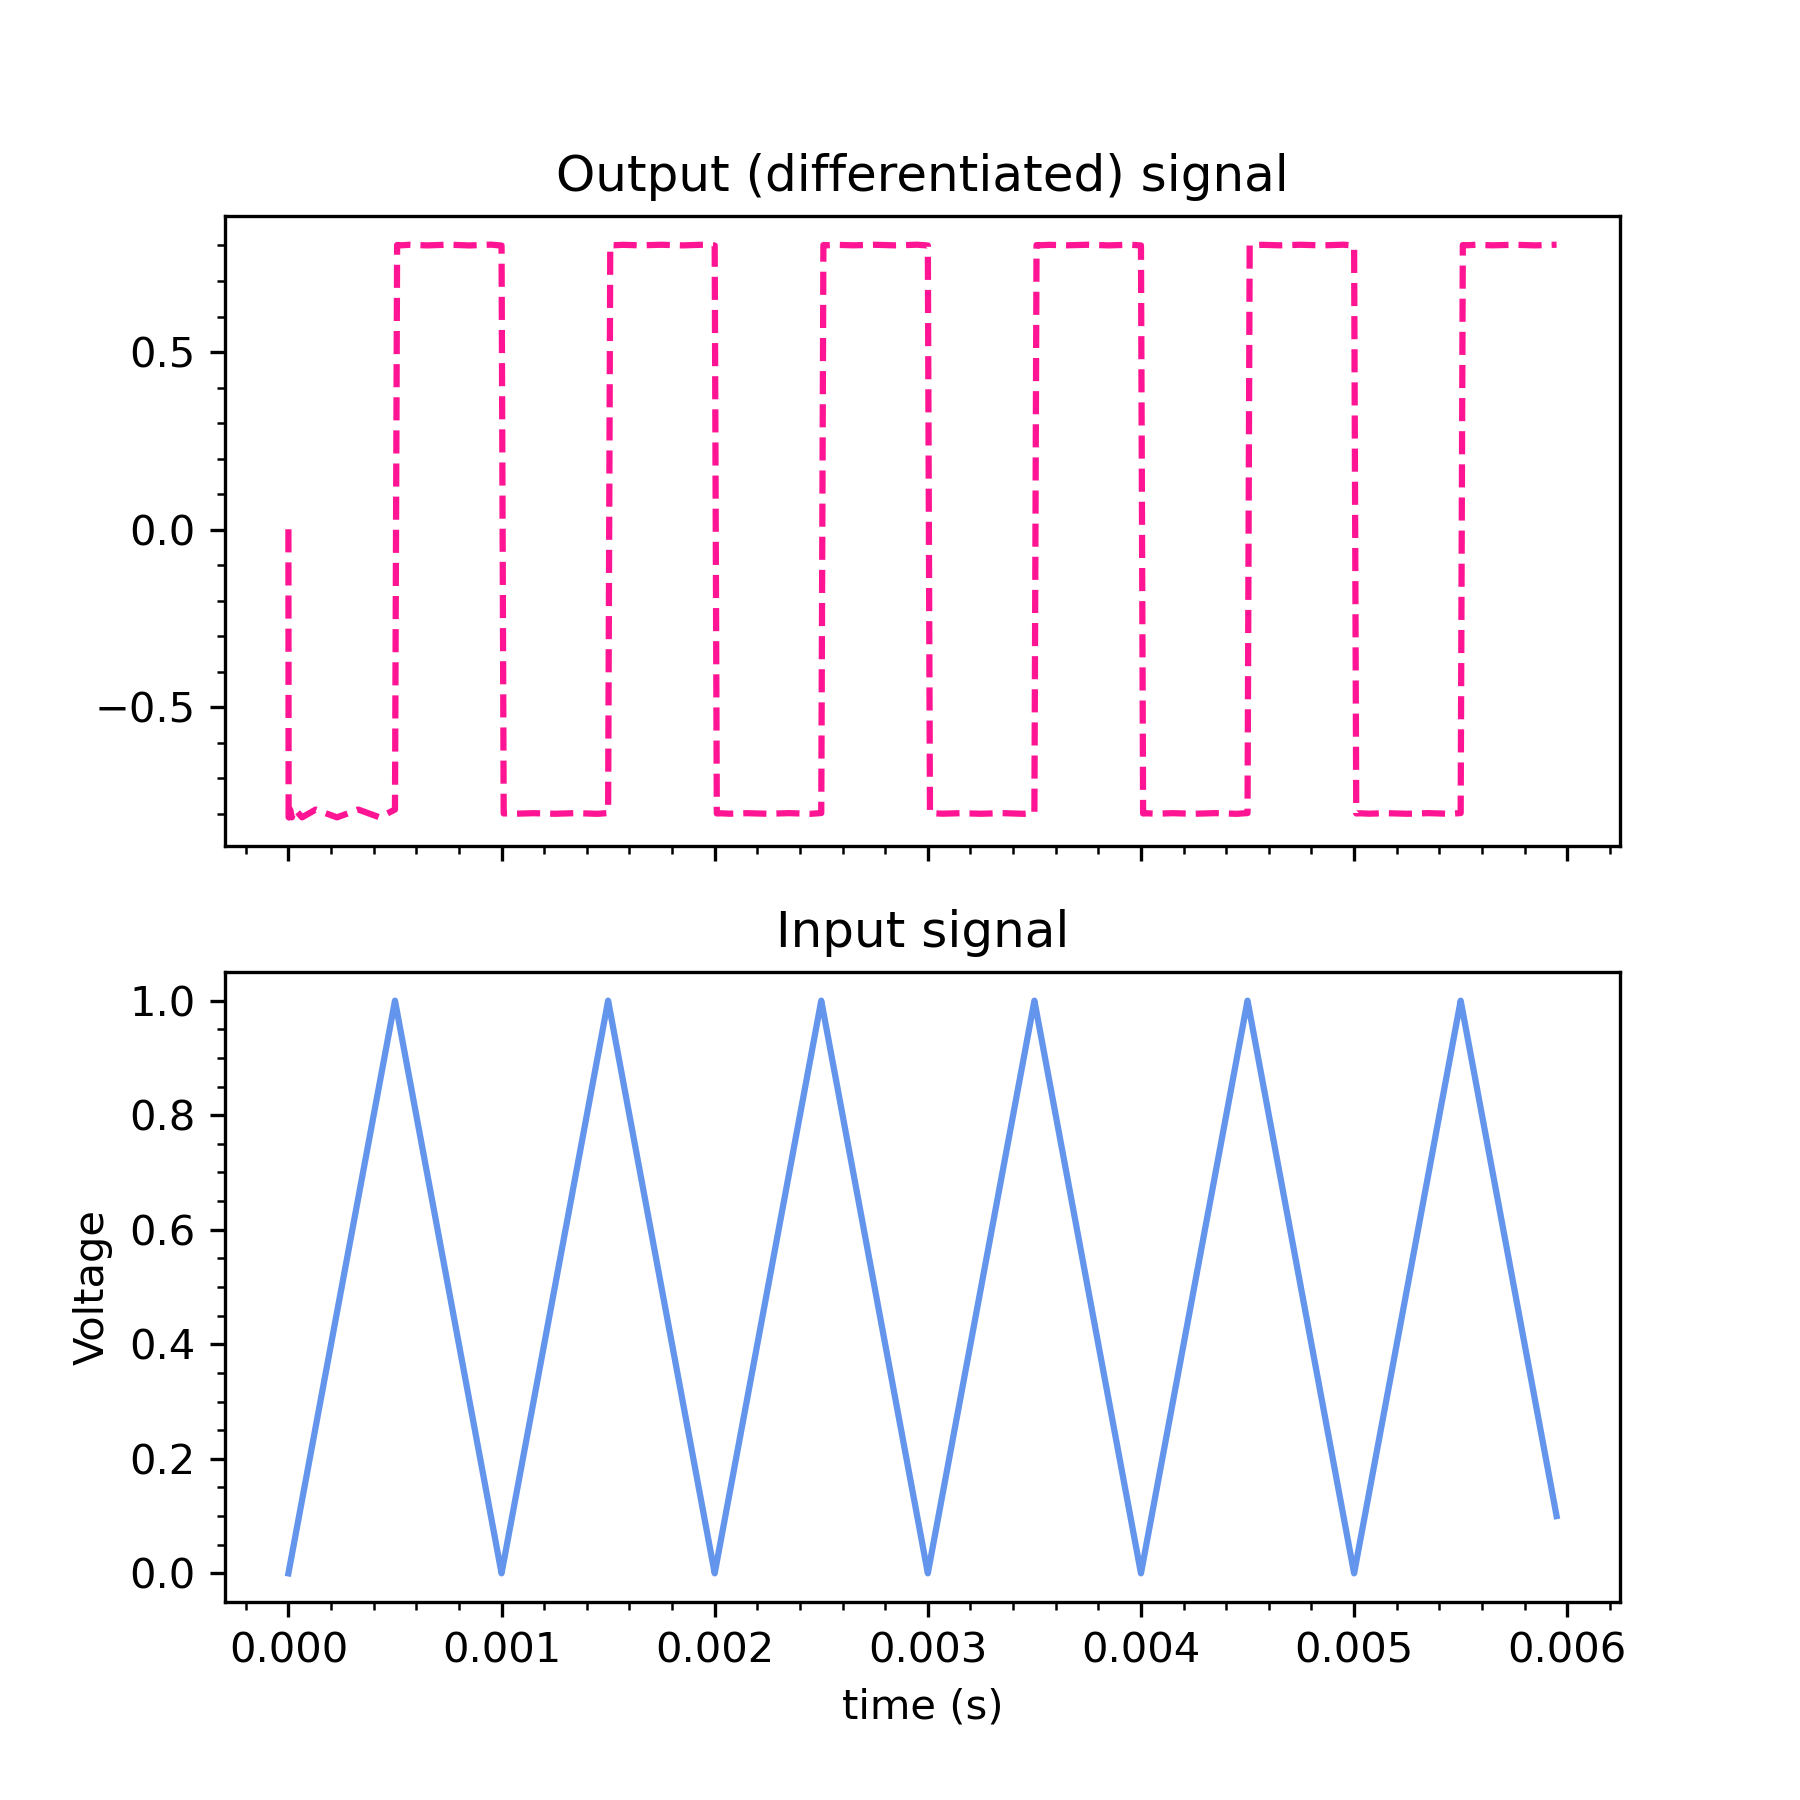
\includegraphics[width=0.5\textwidth]{diff_result}
		\caption{Same as Figure \ref{fig:integ_result} but for the differentiator circuit.}
		\label{fig:diff_result}
	\end{figure}

Therefore, the results are consistent with expectations.

\end{document}